\problemname{Extended Braille}

%\illustration{0.3}{graphic.pdf}{Two characters with the same shape.}
% Source: URL to image.

% optionally define variables/limits for this problem
\newcommand{\maxn}{10^5}
\newcommand{\maxm}{1000}
\newcommand{\maxc}{1000}
\newcommand{\maxdots}{10^6}

The Blind Association for Pretty Calligraphy is annoyed by the lack of emoticons and math symbols in the braille alphabet.
Given that the braille alphabet is supported by the Unicode format,
it only makes sense to make all Unicode characters supported in braille.

The goal is to extend the braille alphabet to include all Unicode characters.
Of course, this will not fit in the standard $2 \times 3$ format, so using a bigger box is allowed.
Important is that no two braille characters are the same up to translation, i.e., have the same shape. See Figure~\ref{fig:braille} for an example.
You let a designer make up a large braille alphabet,
and your job is to check how many unique shapes there are among the characters.

% Given a list of braille characters (by coordinates of their dots),
% find how many of them are unique up to translation (i.e., have a unique shape).

\begin{figure}[h]
    \centering
    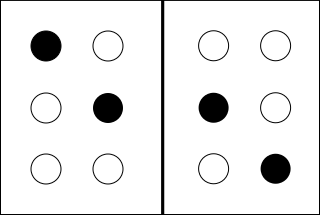
\includegraphics[width=0.3\textwidth]{graphic}
    \caption{Illustration of Sample Input 1:\\two characters with the same shape.}
    \label{fig:braille}
\end{figure}

\begin{Input}
    The input consists of:
    \begin{itemize}
        \item One line with an integer $n$ ($1\leq n\leq \maxn$), the number of braille characters.
        \item Then for each of the $n$ braille characters:
        \begin{itemize}
            \item One line with an integer $m$ ($1 \leq m \leq \maxm$), the number of dots.
            \item $m$ lines, each with two integers $x$ and $y$ ($\left| x \right|, \left| y \right| \leq \maxc$),
            the coordinates of the dots.
        \end{itemize}
    \end{itemize}
    The total number of dots is at most $\maxdots$.
\end{Input}

\begin{Output}
    Output the number of distinct braille characters up to translation.
\end{Output}
